\documentclass{article}

% if you need to pass options to natbib, use, e.g.:
% \PassOptionsToPackage{numbers, compress}{natbib}
% before loading nips_2017
%
% to avoid loading the natbib package, add option 
% \usepackage[nonatbib]{nips_2017}

\usepackage[square,numbers]{natbib}
\bibliographystyle{unsrtnat}

\usepackage{nips_2017}

% to compile a camera-ready version, add the [final] option, e.g.:
% \usepackage[final]{nips_2017}

\usepackage[utf8]{inputenc} % allow utf-8 input
\usepackage[T1]{fontenc}    % use 8-bit T1 fonts
\usepackage{hyperref}       % hyperlinks
\usepackage{url}            % simple URL typesetting
\usepackage{booktabs}       % professional-quality tables
\usepackage{amsfonts}       % blackboard math symbols
\usepackage{nicefrac}       % compact symbols for 1/2, etc.
\usepackage{microtype}      % microtypography
\usepackage{graphicx}
\usepackage{mathtools}
\usepackage{xcolor}
\usepackage{float}
\usepackage{listings}
\usepackage{multirow}
\usepackage{booktabs}

\definecolor{codegreen}{rgb}{0,0.6,0}
\definecolor{codegray}{rgb}{0.5,0.5,0.5}
\definecolor{codepurple}{rgb}{0.58,0,0.82}
\definecolor{backcolour}{rgb}{0.95,0.95,0.92}
 
\lstdefinestyle{mystyle}{
    backgroundcolor=\color{backcolour},   
    commentstyle=\color{codegreen},
    keywordstyle=\color{magenta},
    numberstyle=\tiny\color{codegray},
    stringstyle=\color{codepurple},
    basicstyle=\footnotesize,
    breakatwhitespace=false,         
    breaklines=true,                 
    captionpos=b,                    
    keepspaces=true,                 
    numbers=left,                    
    numbersep=5pt,                  
    showspaces=false,                
    showstringspaces=false,
    showtabs=false,                  
    tabsize=2
}
 
\lstset{style=mystyle}

\title{Optimization of Long Short-Term Memory Networks on GPU}

% The \author macro works with any number of authors. There are two
% commands used to separate the names and addresses of multiple
% authors: \And and \AND.
%
% Using \And between authors leaves it to LaTeX to determine where to
% break the lines. Using \AND forces a line break at that point. So,
% if LaTeX puts 3 of 4 authors names on the first line, and the last
% on the second line, try using \AND instead of \And before the third
% author name.

\author{
  Shuo Niu \\
  University of Toronto \\
  Toronto, Canada \\
  \texttt{shuo.niu@mail.utoronto.ca} \\
  \And
  Li Gu \\
  University of Toronto \\
  Toronto, Canada \\
  \texttt{li.gu@mail.utoronto.ca} \\
  \And
  Yang Fang \\
  University of Toronto \\
  Toronto, Canada \\
  \texttt{jake.fang@mail.utoronto.ca} \\
  %% examples of more authors
  %% \And
  %% Coauthor \\
  %% Affiliation \\
  %% Address \\
  %% \texttt{email} \\
  %% \AND
  %% Coauthor \\
  %% Affiliation \\
  %% Address \\
  %% \texttt{email} \\
  %% \And
  %% Coauthor \\
  %% Affiliation \\
  %% Address \\
  %% \texttt{email} \\
  %% \And
  %% Coauthor \\
  %% Affiliation \\
  %% Address \\
  %% \texttt{email} \\
}

\begin{document}
% \nipsfinalcopy is no longer used

\maketitle
\begin{abstract}
  In this project, we implemented Long Short-Term Memory (LSTM) network on both CPU and GPU, and investigated on optimizations on GPU-level. After all steps of optimizations, our custom cu-LSTM runs as 5.7x speed as GPU baseline, and achieved 163\% bandwidth usage and 580\% floating-point throughput over baseline.  By integrated into applications, our custom cu-LSTM implementation was proved correct with respect to classification accuracy.
\end{abstract}

\section{Introduction}

%%%%%%  Background %%%%%%%%

Recurrent Neural Networks (RNNs) are the state-of-art approaches for a large number of sequence tasks, including sequence generation\cite{eck2002first,sutskever2014sequence,gravessupervised}, machine translation \cite{cho2014learning,jean2015montreal,luong2015effective}, speech recognition \cite{graves2013speech}. LSTM \cite{hochreiter1997long}, an special RNN architecture, can avoid the issue of exploding or vanishing gradient \cite{pascanu2013difficulty} in deeper network and thus be more capable of learning long-term dependencies. A key factor in these recent success has come from the GPUs acceleration \cite{leonard2015rnn,weninger2015introducing} and Nvidia introduces cuDNN library\cite{chetlur2014cudnn} with highly-optimized implementation of RNNs\cite{appleyard2016optimizing} 

%%%%% Method in Brief 
In this project, we learnt GPU programming and optimization techniques in CUDA, and tried to get familiar with several mainstream GPU-accelerated library in deep learning, including cuDNN and Torch. The whole project includes three parts:

% Furthemore, we hope to come up with some strategies to further maximize memory throughput for above existing libraries. 

\begin{itemize}
  \item First, we implemented naive LSTM on CPU and GPU. We analyzed the sequential process of LSTM on CPU and discovered the acceleration provided by pointwise operations on GPU.
  \item Second, we worked on optimizations on GPU level, which further accelerated the naive GPU implementation, expanded bandwidth usage, and increased floating-point throughput. 
  \item Third, we integrated our custom cu-LSTM into PyTorch framework, and compared its performance with PyTorch default CUDA LSTM on application level.
\end{itemize}

%%%%% Evaluation %%%%%%

% To evaluate different optimization strategies, we will have experiments on two different levels: On CUDA level, our implemented optimization strategies will be evaluated with DeepBench\cite{DeepBench}; On application level, we will integrated our custom cuda-LSTM library into PyTorch and evaluate training and inference time in some sequence-to-sequence tasks, such as Neural Machine Translation\cite{luong2015effective}.


% Nvidia introduces the highly optimized cuDNN library\cite{chetlur2014cudnn} in 2014 and brought the support for Simple RNN, GRU, and LSTM architectures in the release of the fifth version in 2016. We would like to implement their unveiled approaches to accelerate a standard LSTM networks and search for the general portable efficient methods for accelerating different forms of RNNs architectures which would be beneficial when implementing and deploying a newly invented RNNs architecture on different GPUs. After investigation of the computation efficiency, we would turn into the memory efficiency of the network which has been significantly overlooked.

\section{Related work}

Recurrent neural networks (RNN) address the problem of recognizing patterns in sequences of data, in the way of looping the same neural network for each sequential input. Inputs along the time sequence relate to each other via multiplication, therefore, derivatives of previous inputs are susceptible to become zero (called vanishing gradient) or infinity (called exploding gradient) in a long input sequence. 

Long Short Term Memory (LSTM)\cite{hochreiter1997long} networks are a special kind of RNN to address the problem of exploding or vanishing gradient when learning long-term dependencies. LSTM cells pass a hidden state in sequence and use four nonlinear functions as gates to decides what information to be forgotten from, added in, or output from the hidden state.

\begin{figure}[h]
\centering
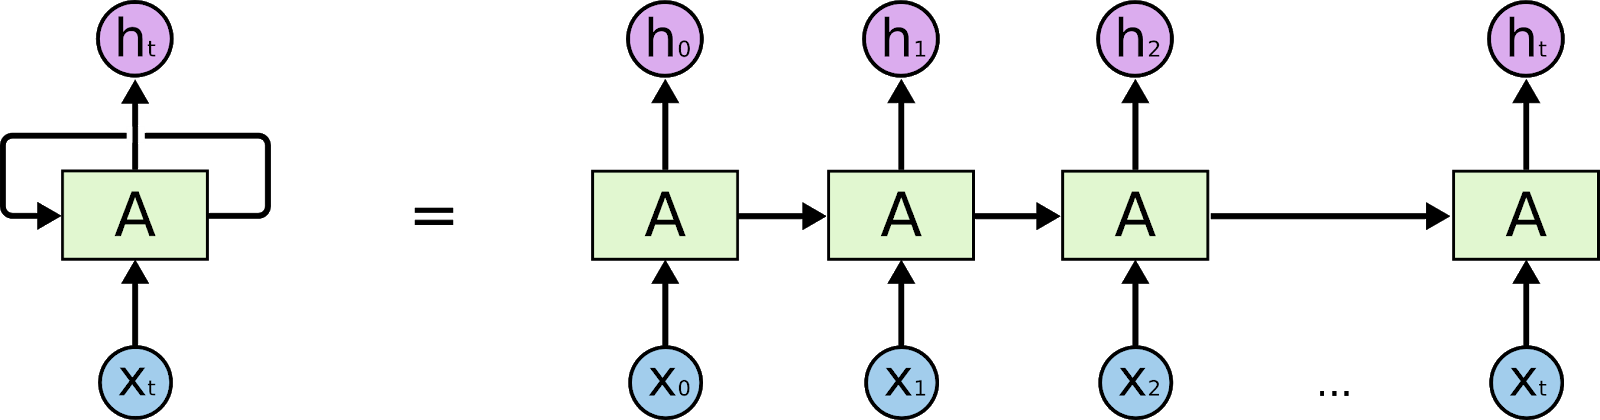
\includegraphics[width=0.7\textwidth]{rnn}
\caption{An unrolled recurrent neural network\cite{understandLSTM}}
\end{figure}

\begin{figure}[h]
\centering
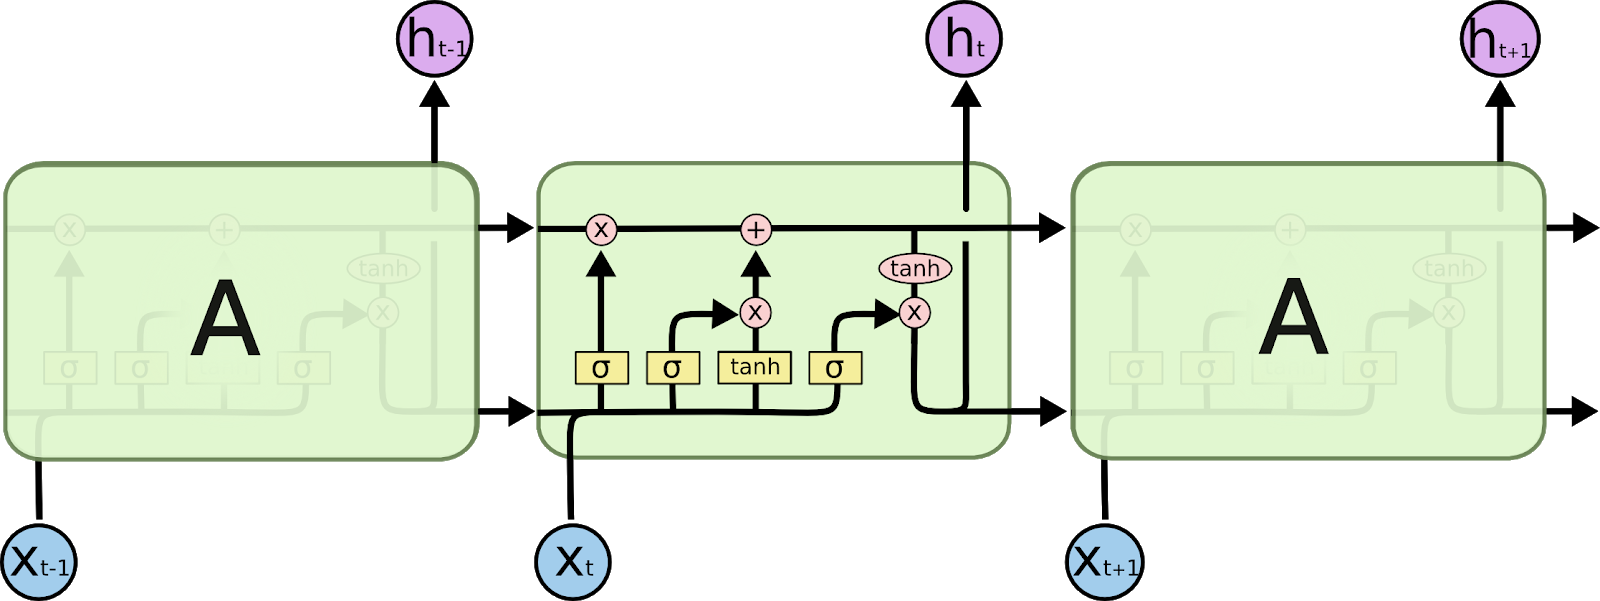
\includegraphics[width=0.7\textwidth]{lstm}
\caption{The repeating module in an LSTM contains four interacting layers\cite{understandLSTM}}
\end{figure}

%%%%% Speed Up %%%%%%%%%%%%%%%%%%%

%% summary of cudnn5
The optimization of LSTM can be implemented on two levels: GPU level and algorithm level. cuDNN\cite{chetlur2014cudnn} is the first library of efficient implementations of deep learning primitives which is easy to integrate into existing frameworks and provides optimized performance and memory usage. Three stages of optimization of LSTM on GPU level was incorporated into cuDNN 5, which achieves an order of magnitude speedup by exposing parallelism between operations.

%% summary on application level 
On algorithm level, exploring alternative architectures to sequence tasks for reducing temporal dependencies and taking the advantage of the parallelism on GPUs have received significant attention recently\cite{chang2017dilated, kaiser2016can, kaiser2015neural, gehring2016convolutional, gehring2017convolutional, kalchbrenner2016neural}. 
\cite{Balduzzi:2016:SRN:3045390.3045527} proposed a recurrent unit with only element-wise linear recurrence relations, which can achieve similar performance to standard non-linear RNNs on text generation.
\cite{bradbury2016quasi} Quasi-RNN has incorporated word-level convolutions into recurrent unit with sequential gated pooling. 
In SRU\cite{lei2017training}, the majority of computation for each step is independent of the recurrence and thus can be easily parallelized, which makes its training as fast as a convolutional layer and 5-10x faster than an optimized LSTM implementation. 
\cite{martin2017parallelizing}abstracts above parallel linear recurrence algorithms and provides an implementation as a CUDA kernel.


%%%%%% Memory usage %%%%%%%%%%%%%%%%%
% \textbf{Reduce Memory Consumption} \\
The trend for deep learning model is to have a “deeper and wider” architecture, which brings the gap between limited GPU device memory capacity and increasing model complexity. Thus, memory optimization becomes a more popular topic in deep learning community. In\cite{chen2015mxnet}, by analysing the data dependencies between operations in a network and allocating the same memory to operations in a network that do not use it concurrently, the memory can be reused.  \cite{gruslys2016memory} exploits dynamic programming to balance a trade-off between caching of intermediate results and recomputation in RNN. On GPU level, \cite{diamos2016persistent} applies the on-chip memory on the GPU to cache the shared RNN parameters during training and optimized barrier implementation on assembly level to reduce the cost of inter-processor synchronization and hide latency, which obtains 16x reduction in memory of activations. \cite{mengtraining} utilizes host memory as a bigger memory pool to overcome the limitation of GPU memory and further proposes a memory-efficient additive attention layer\cite{bahdanau2014neural} for sequence tasks.

%%%% Our job
%The second part in our project is closely related to recent work about optimization memory efficiency on CNN\cite{li2016optimizing}. As the first study to look into the memory efficiency of accelerating CNN on GPUs, they firstly unveiled the impact of data layouts on different types of CNN layers and compare their performance among Alex's cuda-convnet, Caffe and cuDNN. Then, they investigate the internal memory access patterns of the memory-bound layers (pooling and softmax layers) and propose effective optimizations to substantially reduce their off-chip memory requests and internal-kernel communication. Inspired by this work, our project will investigate the memory efficiency of accelerating RNN on GPUs

%%%%% Benchmark
%Baidu DeepBench\cite{DeepBench} is one benchmark that we can use to evaluate our CUDA code on operation-level, particularly dense matrix multiplies, convolutions, and RNN. The metrics it uses are computation time and TeraFLOPS. 
%PyTorch\cite{PyTorch} is a deep learning framework initially released in October 2016, which provides strong GPU acceleration for tensor computation. 
%By employing DeepBench, we will benchmarking our CUDA code against underlying neural network libraries such as cuDNN, and CUDA-Torch, in metrics of time and TFLOPS.

\section{CPU implementation}
For CPU implementation, we use Openblas as our basic linear algebra subprograms library to compute matrix multiplication which is the hot spot of our whole program. We firstly allocate the memory block to store our matrices then we initialize our weights and implement inference as the algorithm showing below which is calculate matrix multiplication for weights and inputs inside every timestep and accross timesteps. After finishing the first layer calculation, we update the matrices and calculate the next layer. Inference time on Intel(R) Core(TM) i7-4790 CPU is 1093.712036ms, with 4 layers, hidden size = 512, batch size = 64, and sequence length = 100. Figure \ref{cell} shows the computation graph of single LSTM cell, and the pseudo code of implementation is present below.

\begin{figure}[H]
\centering
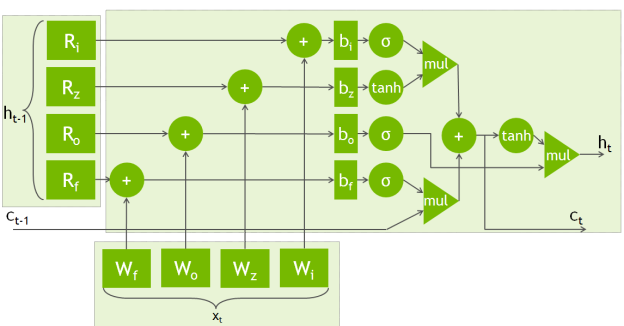
\includegraphics[width=0.7\textwidth]{graph.png}
\caption{Computation graph of single LSTM cell}
\label{cell}
\end{figure}

First, input x and hidden state h from last cell each multiplies with four weight matrices corresponding to four gates. Next, the weighted x and the weighted h are added together, with each gate's bias. Then, they go through four gates' activation functions. Finally, the cell state c and the hidden state h are updated based on both the output from four gates and the cell state passed from last cell.  After updating, cell state and hidden state are passed to the next cell on the same layer.
.
\begin{equation}
  \begin{split}
    & i_t=\sigma(W_i\cdot x_t + R_i\cdot h_{t-1} + b_i) \\
    & z_t=\tanh(W_z\cdot x_t + R_z\cdot h_{t-1} + b_z) \\
    & o_t=\sigma(W_o\cdot x_t + R_o\cdot h_{t-1} + b_o) \\
    & f_t=\sigma(W_f\cdot x_t + R_f\cdot h_{t-1} + b_f) \\
    & C_t=f_t * C_{t-1}+i_t * z_t \\
    & h_t=o_t * \tanh(C_t) \\
  \end{split}
\end{equation}

\begin{lstlisting}[language=Python, caption=Pseudo code of LSTM implementation]
for layer in layers:
    for timestep in timesteps:
        # 1. {input x} and {hidden state h from last cell} each multiplies with four weight matrices corresponding to four gates
        x_forget = x * x_f_weight
        x_input  = x * x_i_weight
        x_cell   = x * x_c_weight
        x_output = x * x_o_weight
        
        h_forget = h * h_f_weight
        h_input  = h * h_i_weight
        h_cell   = h * h_c_weight
        h_output = h * h_o_weight
        
        # 2. add {weighted x} and {weighted h} together before the gates
        forget_gate_input = x_forget + h_forget + bias_forget
        input_gate_input  = x_input  + h_input  + bias_input
        cell_gate_input   = x_cell   + h_cell   + bias_cell
        output_gate_input = x_output + h_output + bias_output
        
        # 3. go through four gates' activation function
        forget_gate_output = sigmoid(forget_gate_input)
        input_gate_output  = sigmoid(input_gate_input)
        cell_gate_output   = tanh(cell_gate_input)
        output_gate_output = sigmoid(output_gate_input)
        
        # 4. pass updated {cell state c} and {hidden state h} to next cell on current layer
        updated_cell_state = (forget_gate_output * cell_state) + 
                             (input_gate_output  * cell_gate_output)
        updated_hidden_state = output_t * tanh(updated_cell_state)
\end{lstlisting}

\section{GPU implementation and optimization}


On GPU, all matrix operations including vector addition, vector multiplication and matrix multiplication can be computed parallelly. Nvidia Visual Profiler shows that in GPU implementation, matrix multiplication takes 90.8\% threads used. Thus, using parallized matrix operations with highly-optimized matrix multiplication function 'cublasSgemm' can achieve 261.399902ms run time, which is 4.2 times faster than CPU implementation, where CPU is Intel(R) Core(TM) i7-4790 and GPU is GeForce GTX 980. 

Nvidia GeForce GTX 980 is used in experiments, which has peak bandwidth - 224 GB/s and peak floating-point throughput - 4.9 TFLOPs. By Nvidia Visual Profiler, it is measured that non-optimized LSTM code achieves only 82 GB/s (36.6\% of peak) and 411 GFLOPs (8.4\% of peak), far from GPU's maximum. Therefore, the non-optimized LSTM is limited by neither bandwidth bound nor compute bound, but latency bound. Latency bound occurs when not much data is used, but it needs to be waited a lot to copy the data from global memory to SMs. 

Techniques that are applied to deal with latency bound includes data prefetching, software pipelining, and to organize the operations in order to make the processor does not stay idle waiting for data. Therefore, there are three general guidelines of optimizations: first, combining small matrices to larger one; second, fusing pointwise operations; third, increasing concurrency.

\underline{\large{Optimization 1: combining weights}}

If a number of independent matrix multiplications share the same input, they can be combined into one larger matrix multiplication which has output of the same times larger. Therefore, four weight matrices that multiply with hidden state and other four weight matrices that multiply with input are combined respectively, leading to the reduction of the number of matrix multiplications from eight to two. Each of the new matrix multiplication is four times larger than the original, and also achieves four times parallelism. This optimization gives 2x speedup over GPU baseline and increases floating-point throughput from 411 GFLOPs to 832 GFLOPs. 

\underline{\large{Optimization 2: combining sequential inputs}}

Similar with combining weight matrices, another way to increase the parallelism of matrix multiplication is combining input form sequential time steps. On the same layer, inputs from different time steps share the same weight matrix, therefore they can be combined. The experiment indicates that with the increasing of the number of inputs being combined, the performance gets better, as shown in Figure \ref{opt2}. 

However, in real-time applications, the whole input sequence usually cannot be accessed, and if achieving higher performance with more inputs combined in a window, the model have to wait for the following time-steps until the window is filled, which produces higher delay time in application. Thus, a trade-off should be considered. In the following experiments, sequential inputs with four timesteps are combined in a window for each weight multiplication, which gives 1.4x speedup over GPU baseline and increases floating-point throughput from 411 GFLOPs to 568 GFLOPs.

\begin{figure}[H]
\centering
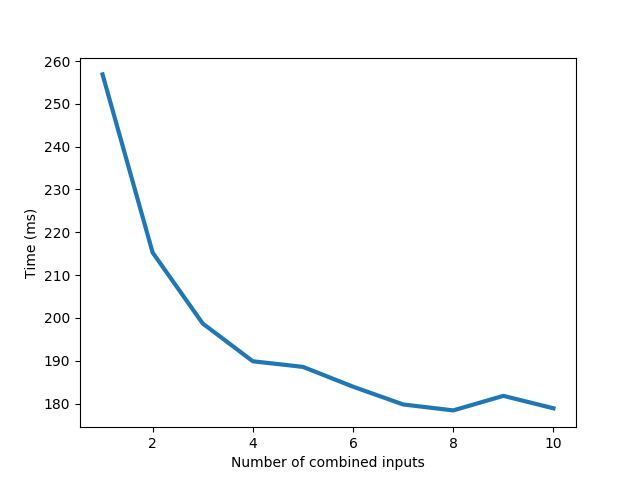
\includegraphics[width=0.5\textwidth]{opt2}
\caption{Number of inputs being combined vs. overall run time (ms)}
\label{opt2}
\end{figure}

\underline{\large{Optimization 3: fusing pointwise operations}}

Nvidia Visual Profiler shows that pointwise operations in separate kernels take up the most of time. By fusing them into one single kernel, data transfer between global memory and threads, and kernel launch overheads are both reduced. This optimization gives 1.2x speedup over GPU baseline, and also increases bandwidth usage from 82 GB/s to 134 GB/s.

\underline{\large{Optimization 4: streaming matrix multiplications}}

The matrix multiplications of hidden state h and input x are independent because they take different weights, hence they can be computed concurrently on separate CUDA streams, which doubles the number of concurrent thread blocks on GPU. The pseudo code shows the way using CUDA event to synchronize both streams. It gives 1.3x speedup of overall runtime over baseline, and increases floating-point throughput from 411 GFLOPs to 528 GFLOPs.

\begin{lstlisting}[language=Python, caption=Pseudo code of using event to synchronize two streams]
cublasSetStream(stream_x); # set stream_x
cublasSgemm(x,x_weights); # do matrix multiplication of x on stream_x
cudaEventCreate(&event_x);
cudaEventRecord(event_x,stream_x); # event_x records stream_x

cublasSetStream(stream_h); # set stream_h
cublasSgemm(h,h_weights); # do matrix multiplication of h on stream_h
cudaStreamWaitEvent(stream_h,event_x); # stream_h waits for the completion of event_x

# After finishing x's multiplication on stream_x and finishing h's multiplication on stream_h, do kernel on stream_h
\end{lstlisting}

\underline{\large{Optimization 5: streaming layers}}

\begin{figure}[H]
\centering
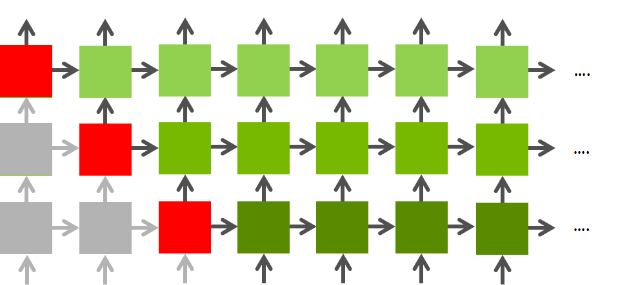
\includegraphics[width=0.7\textwidth]{layers}
\caption{LSTM dependency graph}
\label{dependency}
\end{figure}

Figure \ref{dependency} is the dependency graph of LSTM where one box represents one LSTM cell. The computation of each cell only depends on those of two other cells: the one on the previous time step of the same layer and the one on the same time step of the previous layer. Therefore, one layer can be started before finishing the whole previous layer. By creating CUDA streams for each layer's usage, cells on different layers can run concurrently. So that it achieves the same number times as much parallelism as the number of layers. Figure \ref{opt5} shows with the increasing of the number of layers, the overall run time decreases. 

\begin{figure}[H]
\centering
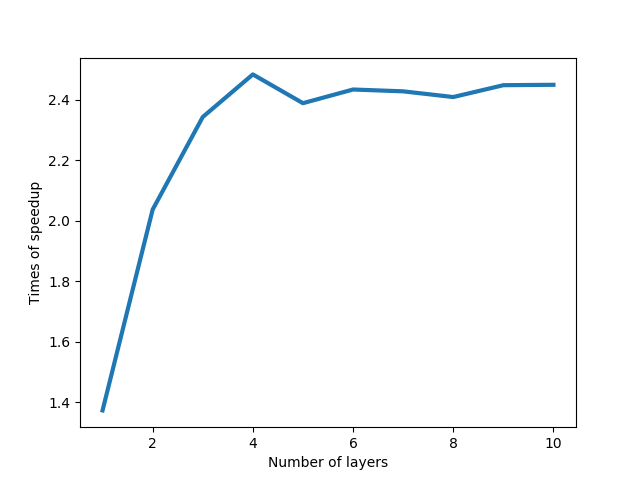
\includegraphics[width=0.5\textwidth]{opt5}
\caption{Number of layers vs. times of speedup after multi-layer optimization}
\label{opt5}
\end{figure}

The pseudo code shows that CUDA event can be used to synchronize the computation on different streams. This multi-layer optimization achieves 2.5x speedup over baseline, and increases floating-point throughput from 411 GFLOPs to 1022 GFLOPs.

\begin{lstlisting}[language=Python, caption=Pseudo code of using event to synchronize multi-layers]
# previous layer
kernel <<< gridDim,blockDim,0,stream_h[layer - 1] >>> (args); # do kernel on stream_h[layer - 1]
cudaEventCreate(&event_h[layer - 1][time_step]);
cudaEventRecord(event_h[layer - 1][time_step],straem_h[layer - 1]);

# current layer
cudaStreamWaitEvent(stream_x[layer],event_h[layer - 1][time_step]);
# After finishing the previous layer's kernel on stream_h[layer - 1], matrix multiplication of input x on the current layer will proceed on stream_x[layer]
\end{lstlisting}

\underline{\large{Experiment results}}

By stacking all five optimizations, our custom cu-LSTM achieves 5.7x speedup over GPU baseline, the bandwidth usage expands to 134 GB/s (59.8\% of GPU's maximum) and the floating-point throughput is increased to 2384 GFLOPs (48.7\% of GPU's maximum). Table \ref{ablation} shows performance of each single optimization as well as performance of the combination of five optimizations.

\begin{table}[H]
\centering
\caption{Ablation study of each optimization}
1. combining weights; 2. combining inputs; 3. fusing pointwise operations; \\4. streaming matrix multiplications; 5. streaming layers
\label{ablation}
\begin{tabular}{|l|l|l|l|l|r|c|c|c|}
\hline
1 & 2 & 3 & 4 & 5 & \multicolumn{1}{l|}{Run Time (ms)} & \multicolumn{1}{l|}{Speedup} & \multicolumn{1}{l|}{BW (GB/s)} & \multicolumn{1}{l|}{GFLOPs} \\ \hline
 &  &  &  &  & 261.399902 & (1.0x) & 82 & 411 \\ \hline
\checkmark &  &  &  &  & 128.755264 & 2.0x & 82 & 832 \\ \hline
 & \checkmark &  &  &  & 188.972900 & 1.4x & 82 & 568 \\ \hline
 &  & \checkmark &  &  & 225.724670 & 1.2x & 134 & 475 \\ \hline
 &  &  & \checkmark &  & 203.495102 & 1.3x & 82 & 528 \\ \hline
 &  &  &  & \checkmark & 104.884064 & 2.5x & 82 & 1022 \\ \hline
\checkmark & \checkmark & \checkmark & \checkmark & \checkmark & 45.466976 & 5.7x & 134 & 2384 \\ \hline
\end{tabular}
\end{table}

Table \ref{cumulative} presents step speedup and cumulative speedup of our five steps of optimization.

\begin{table}[H]
\centering
\caption{Cumulative speedup}
\label{cumulative}
\begin{tabular}{@{}cccc@{}}
\toprule
 & Time (ms) & \begin{tabular}[c]{@{}c@{}}Step\\ speedup\end{tabular} & \begin{tabular}[c]{@{}c@{}}Cumulative\\ speedup\end{tabular} \\ \midrule
\begin{tabular}[c]{@{}c@{}}Non-\\ optimized\end{tabular} & 261.399902 & (1.0x) & (1.0x) \\ \cmidrule(r){1-1}
\begin{tabular}[c]{@{}c@{}}Fused\\ kernel\end{tabular} & 225.731400 & 1.2x & 1.2x \\ \cmidrule(r){1-1}
\begin{tabular}[c]{@{}c@{}}Streaming\\ multiplications\end{tabular} & 148.844391 & 1.5x & 1.8x \\ \cmidrule(r){1-1}
\begin{tabular}[c]{@{}c@{}}Combined\\ inputs\end{tabular} & 134.363037 & 1.1x & 1.9x \\ \cmidrule(r){1-1}
\begin{tabular}[c]{@{}c@{}}Combined\\ weights\end{tabular} & 67.173248 & 2.0x & 3.9x \\ \cmidrule(r){1-1}
\begin{tabular}[c]{@{}c@{}}Streaming\\ layers\end{tabular} & 45.466976 & 1.5x & 5.7x \\ \bottomrule
\end{tabular}
\end{table}

Table \ref{hyperparameter} shows the result of hyperparameter exploration, considering different batch size and sequence length. As batch size decreases and sequence length increases, the speedup performance becomes better. The reason is that GPU baseline with smaller batch size and longer sequence length benefits less from parallelism, so that the effect of optimization is more obvious.

\begin{table}[H]
\centering
\caption{Hyperparameter exploration}
\label{hyperparameter}
\begin{tabular}{l|l|c|c|c|c|}
\cline{3-6}
\multicolumn{2}{l|}{\multirow{2}{*}{}} & \multicolumn{4}{c|}{Sequence length} \\ \cline{3-6} 
\multicolumn{2}{l|}{} & 25 & 50 & 75 & 100 \\ \hline
\multicolumn{1}{|l|}{\multirow{4}{*}{\begin{tabular}[c]{@{}l@{}}Batch\\ size\end{tabular}}} & \multicolumn{1}{c|}{32} & 5.0x & 6.3x & 6.6x & 7.0x \\ \cline{2-6} 
\multicolumn{1}{|l|}{} & \multicolumn{1}{c|}{64} & 4.4x & 5.3x & 5.6x & 5.7x \\ \cline{2-6} 
\multicolumn{1}{|l|}{} & 128 & \multicolumn{1}{l|}{3.0x} & \multicolumn{1}{l|}{3.2x} & \multicolumn{1}{l|}{3.3x} & \multicolumn{1}{l|}{3.4x} \\ \cline{2-6} 
\multicolumn{1}{|l|}{} & 256 & \multicolumn{1}{l|}{2.1x} & \multicolumn{1}{l|}{2.3x} & \multicolumn{1}{l|}{2.3x} & \multicolumn{1}{l|}{2.3x} \\ \hline
\end{tabular}
\end{table}

Considering the data transfer between CPU and GPU, we investigated the effect of pinned memory on data transfer time. When data size is greater than 0.1 MB, pinned memory starts outperforming non-pinned memory, as shown in Figure \ref{pinned}. Following the experimental setups(number of layer=4, hidden size = 512, sequence length=100 and batch size=100 ), our custom cu-LSTM transfers 45 MB of data from CPU to GPU global memory. At this data size, non-pinned memory takes 7.557280 ms on data transfer, while pinned memory only takes 3.780832 ms, which is half of non-pinned memory's duration. In the experiments including comparisons between non-optimized CPU  and GPU implementation, pinned memory is used. 

\begin{figure}[H]
\centering
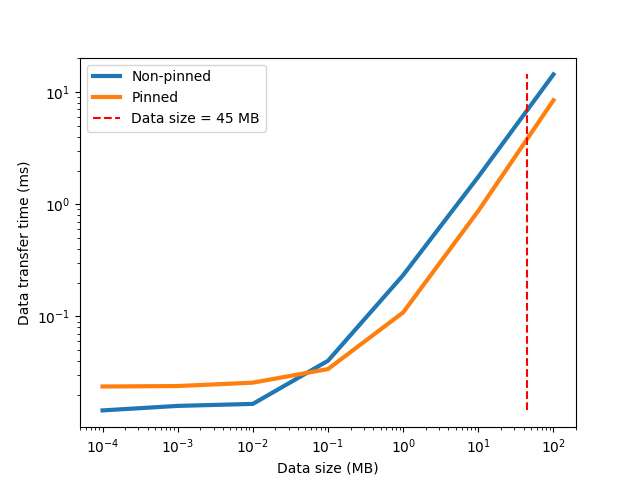
\includegraphics[width=0.7\textwidth]{pinned}
\caption{Comparison of data transfer time from CPU to GPU global memory between using non-pinned memory and using pinned memory}
\label{pinned}
\end{figure}

Compared with cuDNN, the state-of-art GPU-accelerated library for Deep Neural Networks developed by Nvidia, our custom cu-LSTM can achieves 87.4\% of the cuDNN's performance. Experiments are conducted on Amazon Web Service with Intel(R) Xeon(R) CPU E5-2686 and Tesla K80 GPU, and the result is present in Table \ref{benchmark}.

\begin{table}[H]
\centering
\caption{Comparison to benchmark}
\label{benchmark}
\begin{tabular}{@{}l|cccc@{}}
\toprule
 & CPU baseline & GPU baseline & Ours & cuDNN \\ \midrule
\multicolumn{1}{c|}{\begin{tabular}[c]{@{}c@{}}4-layer\\ Hidden size = 512\\ Batch size = 64\\ Length = 100\end{tabular}} & \begin{tabular}[c]{@{}c@{}}3902.052979 ms\\ (1.0x)\end{tabular} & \begin{tabular}[c]{@{}c@{}}398.536682ms\\ 9.8x\end{tabular} & \begin{tabular}[c]{@{}c@{}}90.354431 ms\\ 43.4x\end{tabular} & \begin{tabular}[c]{@{}c@{}}78.935936 ms\\ 49.5x\end{tabular} \\ \bottomrule
\end{tabular}
\end{table}

\underline{\large{Future work on further optimizations}}

From non-optimized LSTM implementation on GPU to our custom cu-LSTM, the bandwidth usage is increased to 59.8\% of GPU's peak, while the floating-point throughput is increased to 48.7\% of GPU's peak, and our cu-LSTM is limited by bandwidth bound and compute bound. Therefore, in future work, overlapping between computing the current batch of data and transfering the next batch of data from CPU to GPU global memory can be used; in addition, persistent RNN \cite{diamos2016persistent} can applie the on-chip memory on the GPU to cache the shared RNN parameters during training.

\section{Applications}

To evaluate the computation correctness of our custom cu-LSTM implementations,  two applications are built on top of the deep learning framework. Deep learning frameworks offer building blocks for designing, training and validating deep learning models, through a high level programming interface. Widely used deep learning frameworks such as Caffe2, Cognitive toolkit, MXNet, PyTorch, TensorFlow  and others rely on its individual GPU-accelerated libraries to deliver high-performance multi-GPU accelerated training and inference. Figure \ref{framework} shows the general stack required for doing deep learning. In this project, PyTorch is used to evaluate our cu-LSTM's performance. Firstly, we have trained a model with PyTorch and saved the model's parameters. Then, the pre-trained model is integrated with PyTorch default LSTM function in CUDA library (cuTorch) and our custom cu-LSTM respectively to do inference on the same test set, and both CUDA implementations adopt single-precision floating-point format. In theory, the application's performance with two implementations should be same.

\begin{figure}[H]
\centering
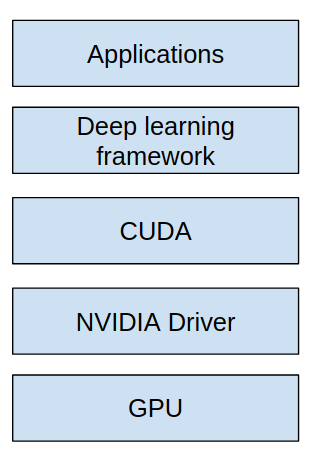
\includegraphics[width=0.25\textwidth]{dependencies.png}
\caption{Deep learning framework Dependencies}
\label{framework}
\end{figure}

The first application is using a character-level LSTM to classify names. A character-level RNN reads one name as a series of characters and produces an output to predict which language the name belongs to. Figure \ref{name-app} have listed several examples. The classification accuracy is used to evaluate the model's performance, as in Table \ref{name-accuracy}, the classification accuracy is evaluated over different batch sizes. To further visualize how well the network performs on different categories,  we have created a confusion matrix as shown in Figure \ref{confusion}, indicating the probability of each language (rows) being categorized by the network to all language categories (columns). The result shows that the model with custom cu-LSTM achieves identical performance with the default PyTorch CUDA library, which proves the correctness of  LSTM in our custom implementation. Additionally, we also evaluate the application's inference times with different batch sizes to compare two LSTM implementations' performance on acceleration. In Figure \ref{name-time}, our cu-LSTM achieves 1.63 times speedup over the PyTorch default LSTM CUDA implementation.

\begin{figure}[H]
\centering
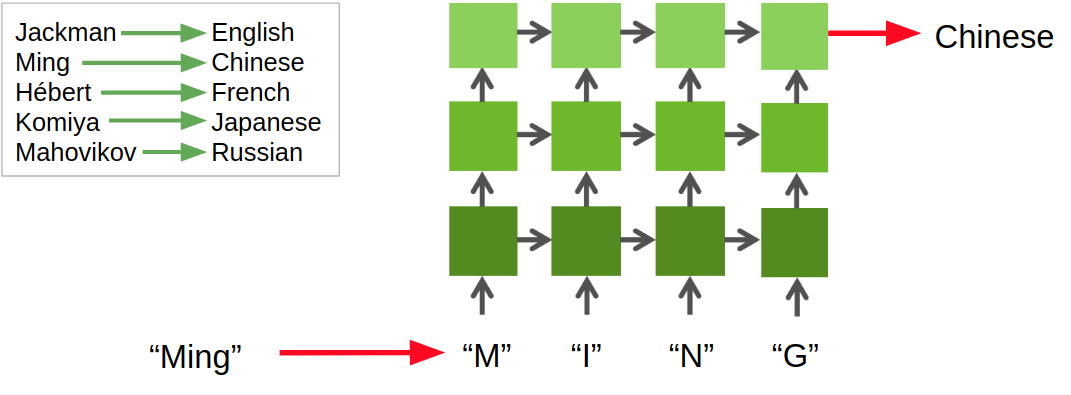
\includegraphics[width=0.9\textwidth]{application.png}
\caption{Classifying names with a character-level LSTM}
\label{name-app}
\end{figure}

\begin{table}[H]
\centering
\caption{Comparison of classification accuracy (\%) of name classification}
\label{name-accuracy}
\begin{tabular}{@{}c|cc@{}}
\toprule
Batch size & Ours & \multicolumn{1}{c}{PyTorch} \\ \midrule
1 & 86.91 & 86.91 \\
3 & 88.58 & 88.58 \\
5 & 88.83 & 88.83 \\
10 & 89.78 & 89.78 \\ \bottomrule
\end{tabular}
\end{table}

\begin{figure}[H]
\centering
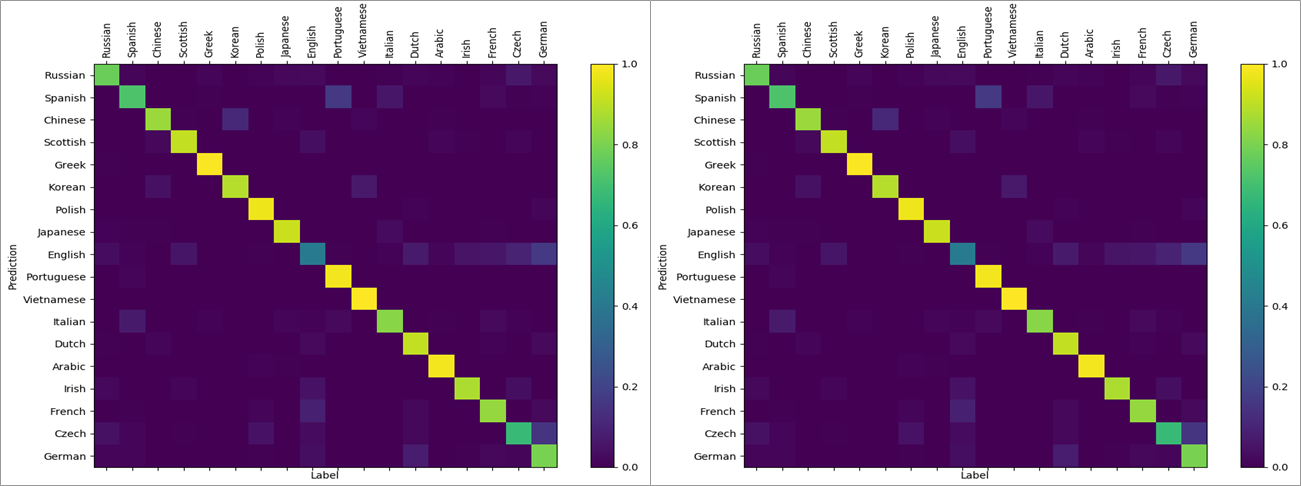
\includegraphics[width=1.0\textwidth]{confusion.png}
\caption{Confusion matrix (left: ours; right: PyTorch)}
\label{confusion}
\end{figure}

\begin{figure}[H]
\centering
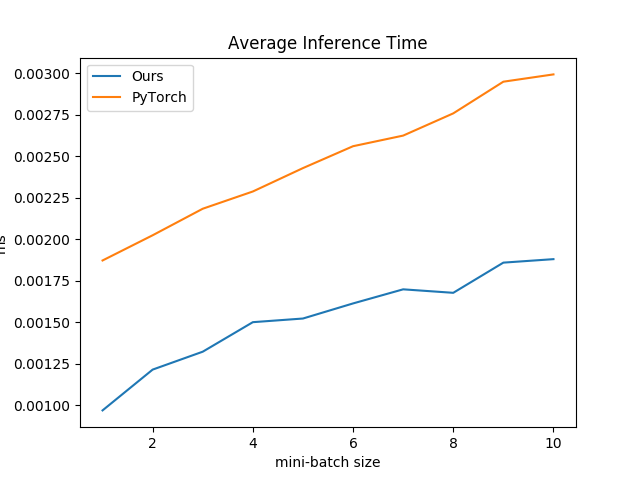
\includegraphics[width=0.65\textwidth]{name.png}
\caption{Inference time of name classification }
\label{name-time}
\end{figure}

The second application is using multi-layer LSTM to classify handwritten digits \cite{deng2012mnist}. each image is in pixel size 28 * 28, and we reshape each image to follow the format of LSTM's input, with hidden size = 28, sequence length = 28 and number of layer = 4. Table \ref{image-accuracy} shows the classification accuracy with two CUDA implementation of different batch sizes and Figure \ref{image-time} shows the inference time with different batch sizes. This application also proves the correctness of our cu-LSTM computation, which achieves 1.19 times speed up over default PyTorch.

By investigating the LSTM implementaion in cuTorch, we found neither streaming matrix multiplications nor streaming layers is considered. Thus, our custom cu-LSTM is faster than default LSTM with cuTorch

\begin{table}[H]
\centering
\caption{Comparison of classification accuracy (\%) of image classification}
\label{image-accuracy}
\begin{tabular}{@{}c|cc@{}}
\toprule
Batch size & Ours & PyTorch \\ \midrule
10 & 94.67 & 94.67 \\
30 & 95.86 & 95.86 \\
50 & 96.21 & 96.21 \\
100 & 97.34 & 97.34 \\ \bottomrule
\end{tabular}
\end{table}

\begin{figure}[H]
\centering
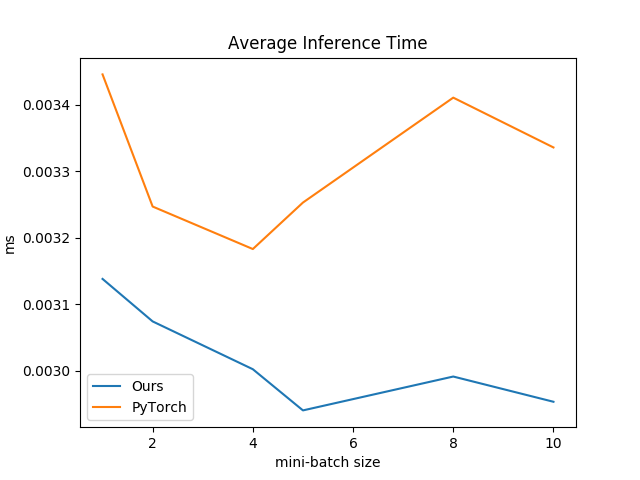
\includegraphics[width=0.65\textwidth]{image.png}
\caption{Inference time of image classification }
\label{image-time}
\end{figure}

\medskip

\section{Conclusion}

Compared with non-optimized GPU implementation of LSTM, by improving latency bound, our custom cu-LSTM achieves 5.7x speed, 163\% bandwidth usage, and 580\% floating-point throughput, which reaches 88\% of cuDNN's performance. Integrated with our custom cu-LSTM, LSTM-based applications built on PyTorch can be faster than those with PyTorch default GPU library, cu-Torch. Our custom cu-LSTM is limited by bandwidth bound and compute bound after optimization, which will be solved in future work.

\bibliography{references}

\end{document}
